\documentclass[oneside,12pt,letterpaper]{article}
\usepackage{graphicx}
\usepackage{latexsym}
%
%---Private Command definitions:
%
\newcommand{\hd}{\mbox{\textsc{hall d}}}
\newcommand{\gx}{\mbox{GlueX}}
%
% DEFINE THE FOLLOWING THREE COMMANDS FOR YOUR GROUP
%
%\newcommand{\instname}{Carnegie Mellon University}
%\newcommand{\groupname}{Medium Energy Physics Group}
%\newcommand{\instabbr}{CMU}
%
%\newcommand{\instname}{Indiana University}
%\newcommand{\groupname}{Indiana}
%\newcommand{\instabbr}{IU}
%
%\newcommand{\instname}{University of Regina}
%\newcommand{\groupname}{SPARRO}
%\newcommand{\instabbr}{Regina}
%
\newcommand{\instname}{Jefferson Lab}
\newcommand{\groupname}{HallD}
\newcommand{\instabbr}{JLab}
%
%---Preamble:
%
\textheight 632pt
\topmargin -0.25truein
%
%---End Preamble.
%
\pagestyle{myheadings}
\markright{\small{\gx{} MOU \\ \instname{} }}
%
\begin{document}

%  #====================#
%---Start the title page
%  #====================#

\begin{center}

\textbf{\large{***DRAFT***DRAFT***DRAFT***\\
Memorandum of Understanding \\ between the 
\gx{} Collaboration, \\ Jefferson Lab \\ and \instname}} \\
18 May, 2004 \\
Draft Version 1
\end{center}

\vspace{1cm}
%  #==================#
%---End the title page
%  #==================#


%  #========================================================#
%---End of preamble, the remainder can be taken as a chapter:
%  #========================================================#

\section{\label{sec:introduction}Introduction}
This Memorandum of Understanding (MOU) outlines the activities and
responsibilities of the \instname{} (\instabbr ) \groupname{} within
the Jefferson Lab (JLab) \gx{} collaboration.  It describes
the commitments of all three parties to the successful completion
of the \gx{} experiment and is subject to regular review and updating
by all three parties. The manpower commitment and deliverables 
described in this document are contingent on continued funding of 
the \instabbr{} group.


The goal of the \gx{} experiment is a mapping of the spectrum of gluonic
excitations with the ultimate objective being a quantitative understanding of
the nature of confinement in QCD.  To achieve this goal a hermetic detector,
the \gx{} spectrometer, optimized for amplitude analysis, will be constructed
in a new experimental hall (\hd ).  A tagger facility will produce 
$9 GeV$ linearly polarized photons via coherent bremsstrahlung radiation 
of $12 GeV$ electrons through a diamond wafer.  To achieve $12 GeV$ 
photons CEBAF will be upgraded to $12 GeV$ with additional cryomodules, 
modified arcs and an additional arc.  Critical Decision 0 (CD-0) for the 
upgrade and \gx{} was awarded by the Department of Energy (DOE) in April, 
2004.  The \gx{} collaboration was formed in 1998.  The fourth and most 
recent version of the \gx{} Design Report was issued in 2002.  The project 
has been reviewed externally and by the JLab PAC.  The \gx{} management 
has been in place since 2000 with a Spokesman, Deputy-spokesman, \hd{} 
group leader and an elected Collaboration Board.


This MOU does not constitute a contractual obligation on the part of 
any collaborating \gx{} institution or JLab. No contractual obligations 
shall arise except pursuant to appropriate written authorizations by each 
party. All foregoing work is subject to the appropriate written contractual 
agreement of the parties.

\section{Institutional Commitments to \gx{} }
In this section we outline the main commitments of \instname{} to the GlueX 
project. The timelines assume that funding will be made available 
as needed, but in practice actual progress will be limited by
external constraints and priorities. 


\subsection{Beamline and Civil Construction}
The construction of the \hd{} beamline, tagger hut, detector
building and counting rooms must come early to allow for efficient
installation and preparation of the experiment.
All necessary ingredients for determining
the parameters for civil construction have been considered and summarized in
some detail in Appendix D of the Design Report. What remains 
is a final review of all components of the design and 
the preparation of a bid package. The schedule for civil construction
is given in Fig.\,\ref{fig:civil_timeline}.


\begin{figure}[h!]\centering

\includegraphics[width=0.75\textwidth]{civil_timeline.pdf}
\caption[]{\label{fig:civil_timeline}
Timeline for civil construction of Hall D beamline, tagger, 
detector and counting room buildings.}
\end{figure}

The JLab accelerator division is responsible for delivery of
the electron beam to the \hd{} beamline. The production,
monitoring and delivery of the coherent photon beam is a joint responsibility
between GlueX, the \hd{} staff and the accelerator. Various
institutions within the \gx{} collaboration (including
the University of Glasgow, University of Connecticut
and Catholic University of America) will contribute to
the production and monitoring of the coherent beam, the design of the tagger magnet, 
collimation and monitoring of the photon beam. A division of
responsibilities and schedule to produce the quality beam
required for the experiment must be made by all contributors.

%\subsection{Beamline}
\subsection{Engineering Design and Safety}
The JLab engineering and design staff will provide support
for many aspects of integration and installation of the
experiment. A complete set of drawings of all components
must reside at JLab for reference and future maintenance.
In particular, the JLab staff is ultimately responsible for
all aspects of safety in \hd{} and must take appropriate
steps to provide training and safe operation of equipment
and healthy environment for personnel.  

\subsection{Solenoid}
The refurbishment of the MEGA/LASS solenoid for use by the 
GlueX experiment is the responsibility of JLab. There are
several modifications which are necessary to update this
magnet for use with a modern experiment. These include
fixing any cryogenic leaks in the four coils, updating
the controls to modern technology, adding iron to the
return yoke for improved magnetic performance, and building
an cryogenic interface to the JLab refrigeration system.
The first task of fixing any problems inside the coils is
being conducted at IUCF in accordance with a MOU (May 16, 2002).
The timeline of this and other work is given
in Fig.\,\ref{fig:solenoid_timeline}. Completion of the 
refurbishment of the magnet, and bringing it into operation
in the new Hall D is a critical-path item, limited presently
by the availability of funding.

\begin{figure}[h!]\centering
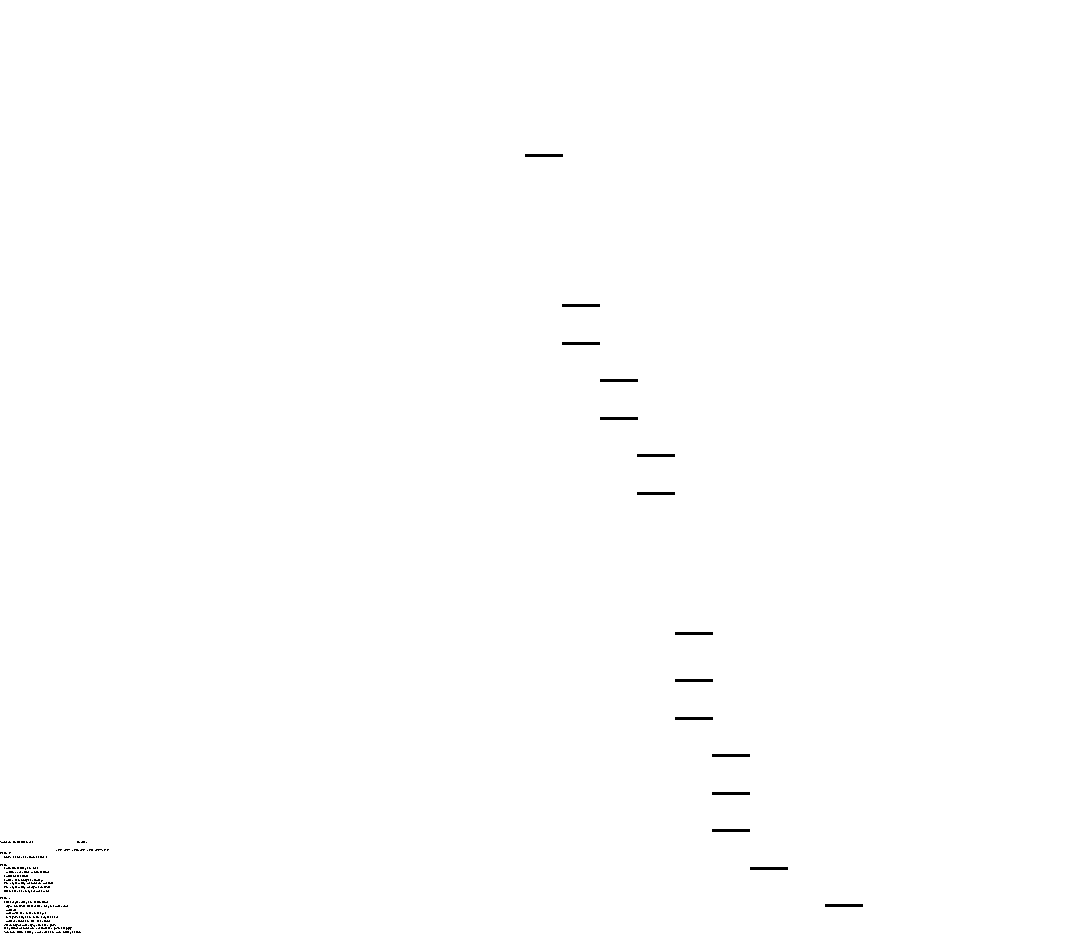
\includegraphics[width=0.75\textwidth]{solenoid_timeline.pdf}
\caption[]{\label{fig:solenoid_timeline} A time line showing the 
overall schedule for the solenoid for Hall D.}
\end{figure}

\subsection{Fast Electronics}
The fast electronics group at JLab is capable of contributing to
several electronics projects for GlueX. The three main tasks that
should be worked on locally are general electrical
infrastructure, a new version of the pipeline TDC, and support for
the Level 1 trigger logic (working closely with David Doughty at
Christopher Newport University). In Fig.\,\ref{fig:electronics_timeline} we
provide a timeline for each of these topics. Additional projects which
the fast electronics group has the expertise to contribute to, in full or in part,
are the development of the Flash ADC board, and front-end electronics.
Based on discussions within the collaboration, we can focus our
efforts on these or other topics. We briefly discuss the three projects
to which we are committed.

\begin{figure}[h!]\centering
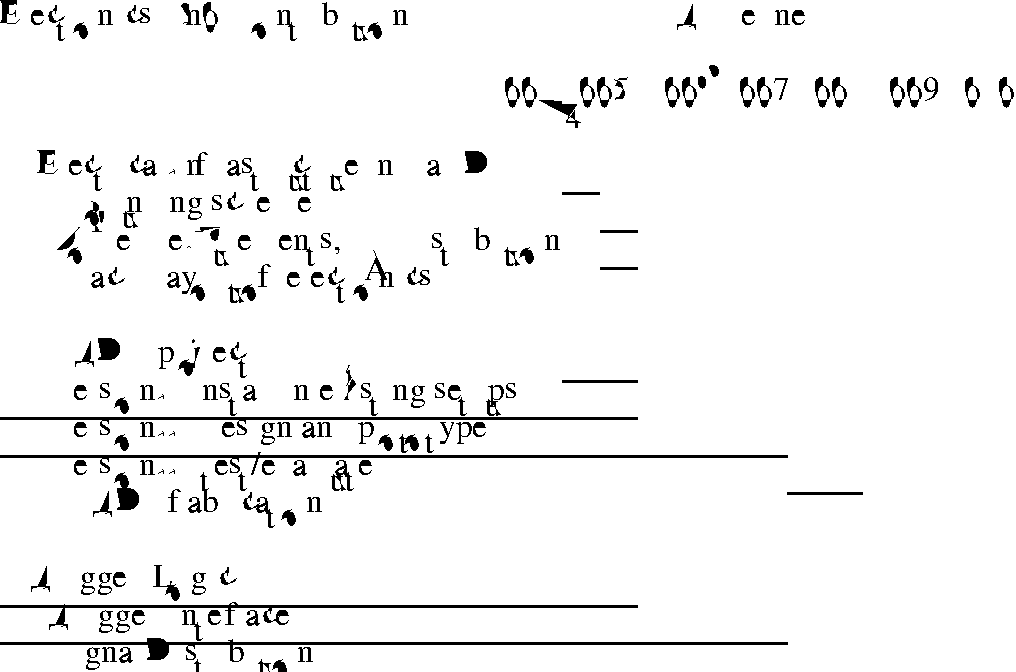
\includegraphics[width=0.75\textwidth]{electronics_timeline.pdf}
\caption[]{\label{fig:electronics_timeline}
Timeline for selected electronic projects to be carried out at JLab.}
\end{figure}

Very soon we need to finalize plans for civil construction. This will
require a grounding plan for the hall, definition of power 
requirements, scheme for the distribution of
clean and dirty AC power, signal conditioning, shielding, etc. This task
needs to be completed early for input to any civil plans for the hall
and is a task which logically falls to local expertise.

The fast electronics group at JLab has developed a TDC board with
64-channels based on the F1 pipeline TDC chip from ACAM. This design
is a significant first step in the development of a module which
satisfies the requirements for time measurements for the GlueX 
experiment. Fifty boards have been fabricated and will be installed
in existing experimental setups at JLab. Based on this experience,
a new board will be developed with all the capabilities required for
GlueX. The proposed timeline for version II of this board is given
in \ref{fig:electronics_timeline}.

The Level 1 trigger is being designed by David Doughty at CNU and
must interface closely to both the DAQ hardware (e.g. trigger
supervisor) and software, as well as to the signal distribution across 
electronic crates. Therefore, the trigger interface and crate-to-crate
communications logically falls
to the fast electronics group and will be developed at JLab.

%\subsection{Target}

\subsection{Data Acquisition}
The data acquisition group is committed to update the JLab CODA 
DAQ framework to accommodate the high data rates required
for the GlueX experiment. These updates will require that
the system be extended to optimize use of pipeline electronics and
associated trigger logic, additional parallel and staged
event builders, and the integration of a software Level 3 farm.
The present runcontrol interfaces, online monitoring, and slow
controls framework will also be integrated for future experiments.
The timeline for this project is given in Fig.\,\ref{fig:daq_timeline}.
The work of the DAQ group needs to be supplemented by a strong
effort within the Hall D group in order to develop
an efficient online system which achieves the goals of
our experiment.

The milestones for this system broadly include the following
\begin{itemize}
   \item Design of clock distribution
   \item Design of new trigger supervisor
   \item CODA upgraded to multiple event builders, now called Event Management Units (EMU),
         but no L3 farm and a single event recorder.
   \item L3 farm version 0 implemented
   \item CODA operational with multiple event builders, L3 farm and multiple event recorders 
\end{itemize}

\begin{figure}[h!]\centering
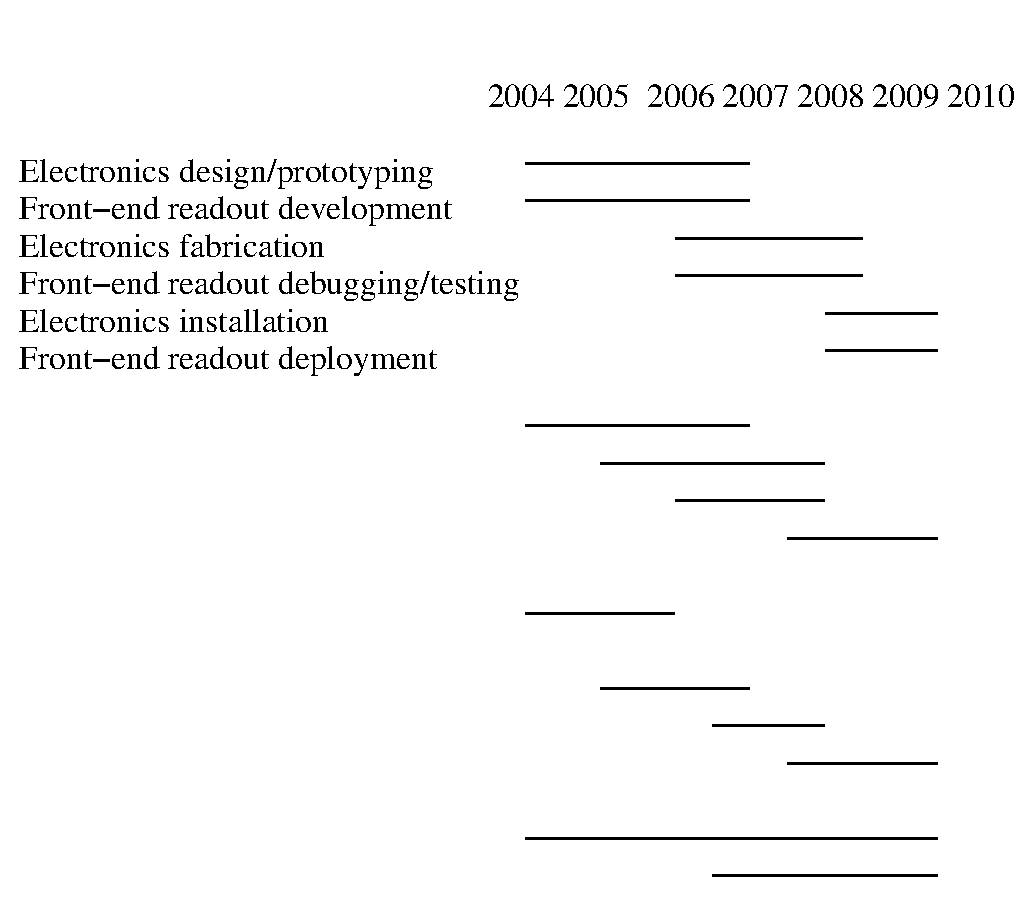
\includegraphics[width=0.75\textwidth]{daq_timeline.pdf}
\caption[]{\label{fig:daq_timeline}A time line showing the 
overall schedule for the GlueX DAQ effort.}
\end{figure}

\subsection{Computing Center Support}
The JLab Computer Center is committed to support the GlueX collaboration by providing data 
storage and reconstruction facilities for Hall D. These facilities will include an integrated 
mass storage system for raw and reconstructed data, an offline batch compute farm, and 
the required infrastructure including high speed networking to support the environment. 
The Computer Center will provide access to these data and compute resources for offsite 
collaborators via a grid enabled framework, as defined through our participation in the 
Particle Physics Data Grid (PPDG) and Open Science Grid (OSG) collaboration efforts.
An initial list of
activities which the computer center is supporting and expects to develop
in the future are given in Fig\,\ref{fig:cc_timeline}.

\begin{figure}[h!]\centering
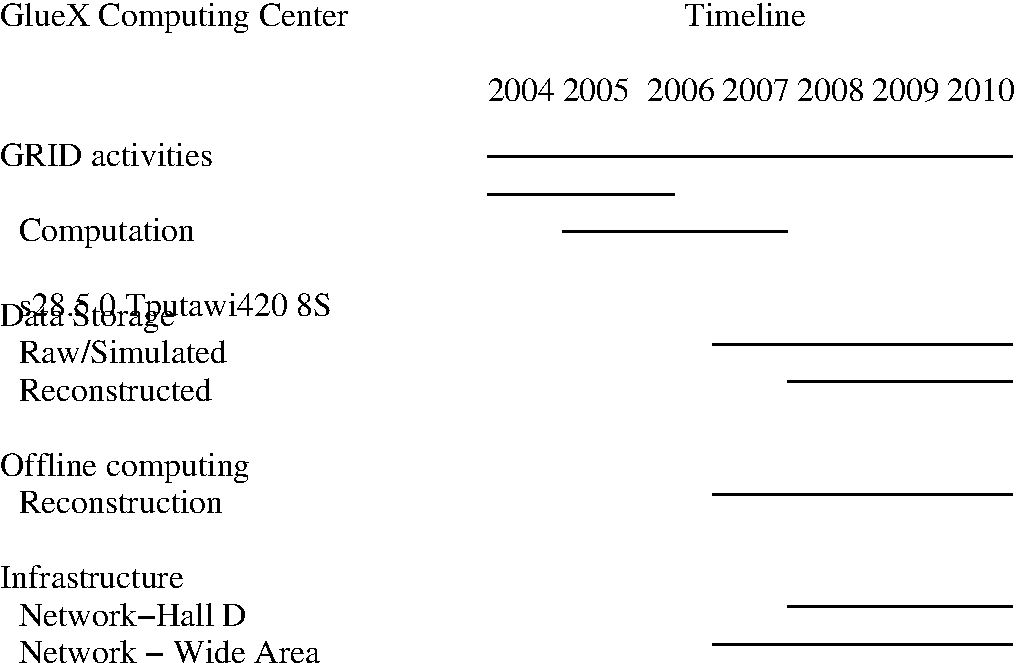
\includegraphics[width=0.75\textwidth]{cc_timeline.pdf}
\caption[]{\label{fig:cc_timeline} A time line showing the 
timeline for various activities by the computing
center in support of GlueX.}
\end{figure}

%\subsection{Hardware Deliverables for \gx{} }

\subsection{Software Deliverables and Support for \gx{} }
%\subsection{Computing and Software}
The primary responsibilities of JLab to the software effort will
be to provide the underlying infrastructure which begins with the efficient
collection of data to the production of reconstructed data. 
This is designated in Fig.9.1 of the design report as ``JLab infrastructure.''
This framework begins the the DAQ system, described
above, followed by integration provided by Hall D personnel and supported
by the JLab computer center staff to provide a productive environment
for offline computing. Some of the tasks which are part of the 
support required are given in Fig.\,\ref{fig:computing_timeline}. 

\begin{figure}[h!]\centering
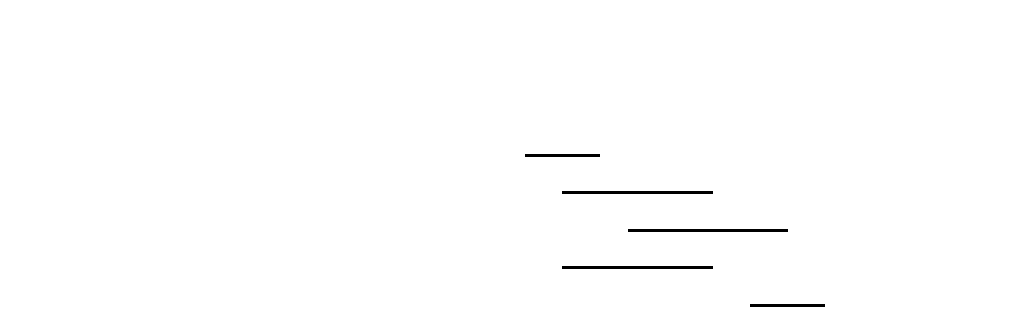
\includegraphics[width=0.75\textwidth]{computing_timeline.pdf}
\caption[]{\label{fig:computing_timeline} A time line showing the
selected topics contributing to the GlueX software effort by
JLab.}
\end{figure}


\subsection{Support for Running The \gx{} Experiment}
%
% This includes maintaining detector components, serving as experts
% on call for various parts of the detector as well as normal shift
% assignments.
%
\subsection{Support for Analysis of \gx{} Data}
%
% This includes calibration of detectors, data quality checks 
% and data processing and management tasks.
%
\subsection{Theoretical Support to \gx{}}
%
% This section describes theoretical calculations relevant to 
% GlueX as well as lectures to educate GlueX collaboration
% members.
%
\subsection{Collaboration Responsibilities}
% 
% This sections describes management roles played by group members.
% It also includes committee memberships that are purely in support
% of the functioning of the experiment. This might include publication
% or speakers committees.
%
Elton Smith currently serves as the Physics Division Liaison for the \gx{}
collaboration. The \instabbr{} group fully supports this effort and
any other efforts deemed necessary by the collaboration. 
%
%\clearpage
\section{Funding and Infrastructure}
\subsection{\instname{}}

The proposal for the 12-GeV upgrade includes the hire of sufficient personnel
to support the construction and maintenance of a new experimental facility
to house the GlueX experiment. The \hd{} group will require 
staffing comparable to existing halls, or approximately 13 persons. In addition,
technical staff for support of this effort is also required, and needs to be
allocated to existing groups within the Physics Division. The
rate of hires and final staffing levels are under discussion between JLab
and the Department of Energy.

\instname{} is committed to support all activities which are required to achieve
a successful experimental program in \hd{}. Resources of infrastructure and
personnel will be made available based on priorities of the 12-GeV program. 

The \instname{} group will provide written time lines for the completion of
various phases of the project and written reports on the outcome of each
of these various phases.

\subsection{The \gx{} Collaboration}

The construction of these projects are contingent
on securing additional funds specifically for this
project. The \gx{} collaboration will develop a global plan for the 
timely funding and construction of all elements of the \gx{} detector. 
The collaboration as a whole will seek funds to build all parts of the
detector in a coordinated fashion.

\subsection{Jefferson Lab}
~\\*[0.25cm]
Note: This section of the MOU is not meaningful for \instname, but has been
left unchanged to conform with other collaboration documents.
~\\*[0.25cm]
\begin{itemize}
\item JLab will retain ownership of all deliverables as specified 
under individual contracts and MOUs.
\item JLab is responsible for all engineering aspects of \gx{} and 
all aspects of the detector integration that require legal and certified
engineer approval.
\item JLab assumes all legal liabilities related to \instabbr{} provided
and installed equipment while located on JLab property.
\item JLab will provide reasonable assistance to the \instabbr{} group
to assure smooth flow of information regarding DOE procedures and 
protocols as they affect the funding of the work agreed between JLab
and \instname .
\item JLab will provide physical space to \instabbr{} personnel and for
their equipment to facilitate their work on \gx . The \instabbr{} group
will convey such requirements to JLab with reasonable advance notice
in the spirit of good relations and sound planning.
\item Official contact between the \instabbr{} group and JLab will be 
through the \hd{} project management office and its JLab appointed staff.
\end{itemize}

\section{\label{sec:personal}Personal}
\begin{flushleft}
1. The contact person for the \instname{} group is Elton Smith. \\
2. The following personnel are included in the \instabbr{} \gx{} group: 
\end{flushleft}
\begin{table}[h!]
\begin{center}
\begin{tabular}{llc} \\
\textbf{Group} & \textbf{Person} & \textbf{Percent of Research Effort} \\
%Accelerator        & Swapan Chattopadhyay	& 15\%   \\
Computing Center   & Graham Heyes   	        & 10\%   \\
Data Acquisition   & David Abbott               & 25\%  \\
Data Acquisition   & David Lawrence             & 80\%  \\
Data Acquisition   & Ed Jastrzemski		& 25\%   \\
Data Acquisition   & Elliott Wolin		& 50\%   \\
Data Acquisition   & Vardan Gyurjyan		& 25\%   \\
Detector           & Brian Kross		& 50\%   \\
Detector           & Stan Majewski		& 20\%   \\
Detector           & Vladimir Popov		& 35\%   \\
Detector           & Drew Weisenberger		& 15\%   \\
Detector           & Ben Welch		        & 25\%   \\
Detector           & Randy Wojcik		& 50\%   \\
Detector           & Carl Zorn 		        & 50\%   \\
Engineering        & Paul Brindza               & 25\%   \\
Engineering        & Ravi Anumagalla            & 100\%   \\
Fast Electronics   & Chris Cuevas		& 15\%  \\
Fast Electronics   & Fernando Barbosa		& 25\%  \\
Fast Electronics   & James Proffitt		& 15\%  \\
Hall B             & Elton Smith                & 50\%   \\
Hall B             & Dennis Weygand             & 10\%  \\
Hall C             & Steve Wood		        & 15\%   \\
%Hall C             & Roger Carlini              & 15\%   \\
Hall C             & Howard Fenker              & 15\%   \\
Theory             & Andrei Afanasev            & 15\%   \\
Theory		   & Wally Melnitchouk		& 15\%   \\
\end{tabular}
\caption[]{\label{tab:halldpersonnel} ***DRAFT***DRAFT***
The percentages refer to the approximate percentage of research time to be
spent by the person on all \gx{} activities during FY2004--FY2006 time
period. These commitments will be updated as the project matures.}
\end{center} 
\end{table}

\section{Special Considerations}
\begin{enumerate}
\item[1] The \gx{} collaboration will have final responsibility for 
the acceptance of all deliverables and retains the right, to terminate 
or renegotiate this MOU if the technical requirements, performance, 
physical specifications, time schedules and costs cannot be met by the 
\instname{} group.
\item[2] The \gx{} collaboration retains the right to assign additional
manpower and/or additional groups to this project if it is deemed that
this is necessary for timely and within budget completion of the project.
\item[3] The continuation of this agreement is dependent on the approval 
for continuing  funding for all parties in the MOU.
\item[4] This agreement may be amended as necessary.
\item[5] The \instname{} group, the \gx{} Collaboration management and the 
JLab management of \gx{} agree to commit themselves on a collegial, open and
effective working relationship for the benefit of the project.
\end{enumerate}

\bibliography{mou}
\bibliographystyle{unsrt}

\clearpage
\begin{center}\textbf{SIGNATURE PAGE}\end{center}
%
% We should have the minimum number of signatures possible. This
% should include the institution representative(s), The collaboration
% spokesperson and either the JLab Group Leader or Larry Cardman.
%
\begin{tabbing}
\=ChairxofxthexCollaborationxBoardxxxxxxxxx\= \kill
\\
\\
\\
\> \_\_\_\_\_\_\_\_\_\_\_\_\_\_\_\_\_\_\_\_\_\_\_\_\_\_\_\_\_\_\_\_\_\_\_\_ 
\> \_\_\_\_\_\_\_\_\_\_\_\_\_\_\_\_\_\_\_\_\_\_\_\_\_\_\_\_\_\_\_\_\_\_\_\_
\\
\>Dr. Elton S. Smith \> Date \\
\>Physics Division Liaison \hd{} \\
\> \instname{}  \\
\\
\\ 
\\
\> \_\_\_\_\_\_\_\_\_\_\_\_\_\_\_\_\_\_\_\_\_\_\_\_\_\_\_\_\_\_\_\_\_\_\_\_ 
\> \_\_\_\_\_\_\_\_\_\_\_\_\_\_\_\_\_\_\_\_\_\_\_\_\_\_\_\_\_\_\_\_\_\_\_\_ 
\\
\> Prof. Alex Dzierba           \> Date \\
\> Spokesperson                 \\
\> \gx{} Collaboration          \\
\\
\\
\\
\> \_\_\_\_\_\_\_\_\_\_\_\_\_\_\_\_\_\_\_\_\_\_\_\_\_\_\_\_\_\_\_\_\_\_\_\_ 
\> \_\_\_\_\_\_\_\_\_\_\_\_\_\_\_\_\_\_\_\_\_\_\_\_\_\_\_\_\_\_\_\_\_\_\_\_ 
\\
\> Dr. Larry Cardman \> Date \\        
%\> Dr. Elton Smith \> Date \\
\> Associate Director for Physics \\ 
%\> JLab \hd{} Group Leader \\
%\> Jefferson Lab                   
\> Jefferson Lab \\
%
\end{tabbing}
\end{document}






